% Chapter Template

\chapter{Swarm} % Main chapter title

\label{Chapter2} % Change X to a consecutive number; for referencing this chapter elsewhere, use \ref{ChapterX}

\lhead{Capítulo 2. \emph{Swarms}} % Change X to a consecutive number; this is for the header on each page - perhaps a shortened title

%----------------------------------------------------------------------------------------
%	SECTION 1
%----------------------------------------------------------------------------------------

\section{Comportamiento colectivo en la naturaleza}

\begin{figure}[htbp]
	\centering
		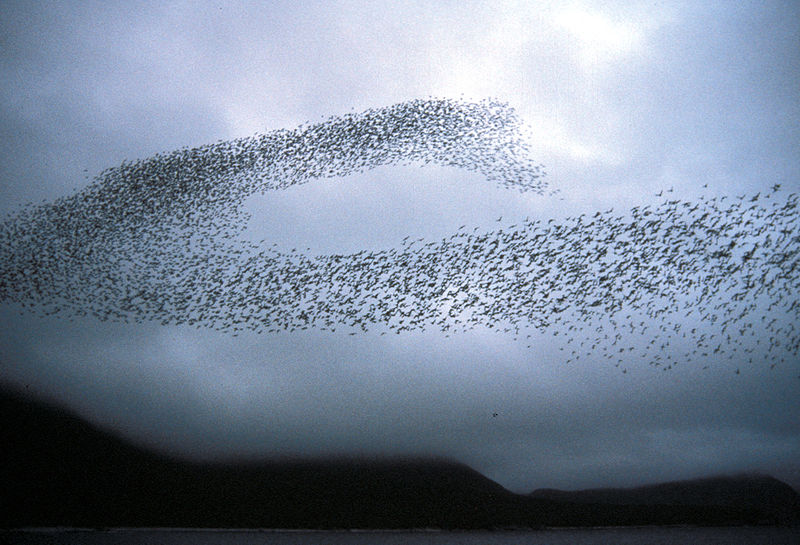
\includegraphics[width=0.8\textwidth]{./Figures/swarm.jpg}
		\rule{35em}{0.5pt}
	\caption[swarm]{Bandada de auklets, teniendo comportamiento de enjambre. Imagen extraida de Wikipedia.}
	\label{fig:swarm}
\end{figure}

Existen casos de enjambres, los más típicos son las hormigas y abejas, pero los hay en peches, aves e incluso los mamíferos. Son sistemas donde nadie está a cargo y aún así ejecutan una tarea grupal. Las hormigas son un gran ejemplo. Al momento de construir su nido, no tienen un arquitecto o ingeniero estructural que esté dando órdenes, simplemente cada una sabe que tiene que hacer. No hay un director orquestando la construcción desde lo alto, en vez de esto lo que ocurre es un comportamiento emergente. También conocido como inteligencia de enjambre.

Otro tipo de comportamiento colectivo son las migraciones, desplazamientos periódicos que efectúan aves, peces, langostas y mamíferos de un hábitat a otro. Cada individuo activo en la migración sigue al grupo, los más pequeños como el plancton o anfibios aprovechan las corrientes de aire o agua, y las aves, más grandes, aprovechan los vientos y corrientes ascendentes. Hay diversas finalidades detrás de la migración, algunas especies lo hacer para escaparse de los crudos inviernos o secos veranos; mientras que otras, como las tortugas marinas, por una necesidad reproductiva emprenden un largo viaje de más de 10.000 millas, a lo largo de todo el Atlántico Norte.

Lograr que un enjambre de robots tenga un comportamiento emergente como el de las colonias de abejas es la piedra filosofal de los investigadores de esta área. Uno de los más destacados investigadores del área, James McLurkin, experto en robótica del Massachusetts Institute of Technology (MIT) dice que para lograrlo es necesario un software que ejecute tareas individuales y     que de alguna forma se cumpla con una tarea grupal. He aquí una importante razón para desarrollar estudios sobre enjambres de robots, ya que aún no está claro cómo se coordina la naturaleza para llevar a cabo tales tareas.

%-----------------------------------
%	SECTION 2
%-----------------------------------
\section{Robots para construir un enjambre}

Imaginemos una situación hipotética donde un edificio es destruido, la búsqueda de sobrevivientes no es una tarea fácil, implica que rescatistas ingresen al lugar corriendo grave peligro, usualmente buscando a las víctimas en condiciones de poca visibilidad. Esto mismo podría ser ejecutado por un enjambre robótico que esté programado para buscar gente y que de manera colectiva recorra un área mucho mayor que 2 o 3 personas. Incluso un robot del mismo enjambre puede fallar, pero al ser un sistema distribuido el enjambre continúa funcionando, es un sistema muy robusto.

A continuación algunos robots que pueden ser utilizados para hacer un Robot Swarm junto con las información técnica disponible.

%-----------------------------------
%	SUBSECTION 1
%-----------------------------------

\subsection{Kilobot}
El proyecto Kilobot, es un sistema de bajo costo escalable para demostrar comportamientos colectivos. Actualmente existen varios grupos que están investigando algoritmos para enjambres de robots, por esto que diseñaron Kilobot que es un robot de bajo costo, accesible,  que permite hacer pruebas en cientos o miles de robots.

\begin{figure}[htbp]
	\centering
		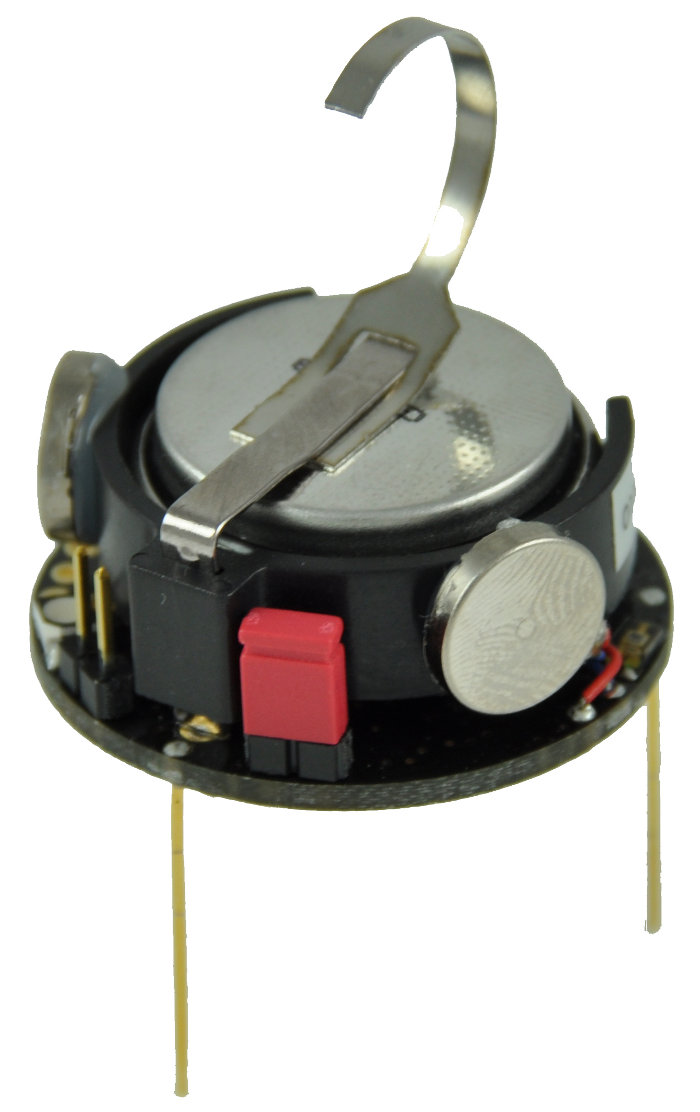
\includegraphics[width=0.4\textwidth]{./Figures/kilobot.jpg}
		\rule{35em}{0.5pt}
	\caption[swarm]{Kilobot. Imagen extraida de http://www.k-team.com.}
	\label{fig:kilobot}
\end{figure}



%-----------------------------------
%	SUBSECTION 2
%-----------------------------------

\subsection{Organismo Multibot}

S. Kornienko, O. Kornienko, A. Nagarathinam y P. Levi., exploran el trabajo colaborativo en robots para un mejor rendimiento y mayor fiabilidad a nivel macroscopico. En este articulo demuestran sus últimos trabajos en sistemas colectivos y lo más sorprendente es que logran la agregación y desagregación autónoma para así obtener un organismo multibot.
\cite{5359578}

\begin{figure}[htbp]
	\centering
		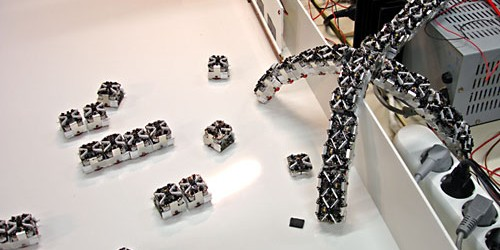
\includegraphics[width=0.7\textwidth]{./Figures/Multibot_organism.jpg}
		\rule{35em}{0.5pt}
	\caption[swarm]{Organismo Multibot. Imagen extraida de http://ieeesbcet.org/}
	\label{fig:Organismo}
\end{figure}


%-----------------------------------
%	SUBSECTION 3
%-----------------------------------

\subsection{E-puck}

Uno de los robots más utilizados por los científicos en el mundo para estudios y publicaciones es el E-puck. Este robot es compacto, tiene forma de cilindro con un diámetro de 7 [cm] y para moverse hace uso de sus dos ruedas, dejándolo en la categoría de robot con desplazamiento diferencial. Originalmente fue diseñado para educar en el área de la micro ingeniería por Michael Bonani y Francesco Mondala en el laboratorio ASL del Profesor Roland Siegwart en Escuela Politécnica Federal de Lausana (EPFL) en Suiza. El e-puck es open hardware, software es de código abierto,  lo construyen y venden varias empresas. Para comunicarse con una computador incorporan un módulo Bluetooth conectado a uno de sus dos puertos serie. Existen varios tipos de accesorios, entre los que destacan un Zigbee para comunicaciones, un módulo con varias cámaras y LEDs RGB como sistema de comunicación visual. Su precio a la fecha en Gctronic es 912 USD. Para comprarlo hay que encargarlo desde Suiza.

\begin{figure}[htbp]
	\centering
		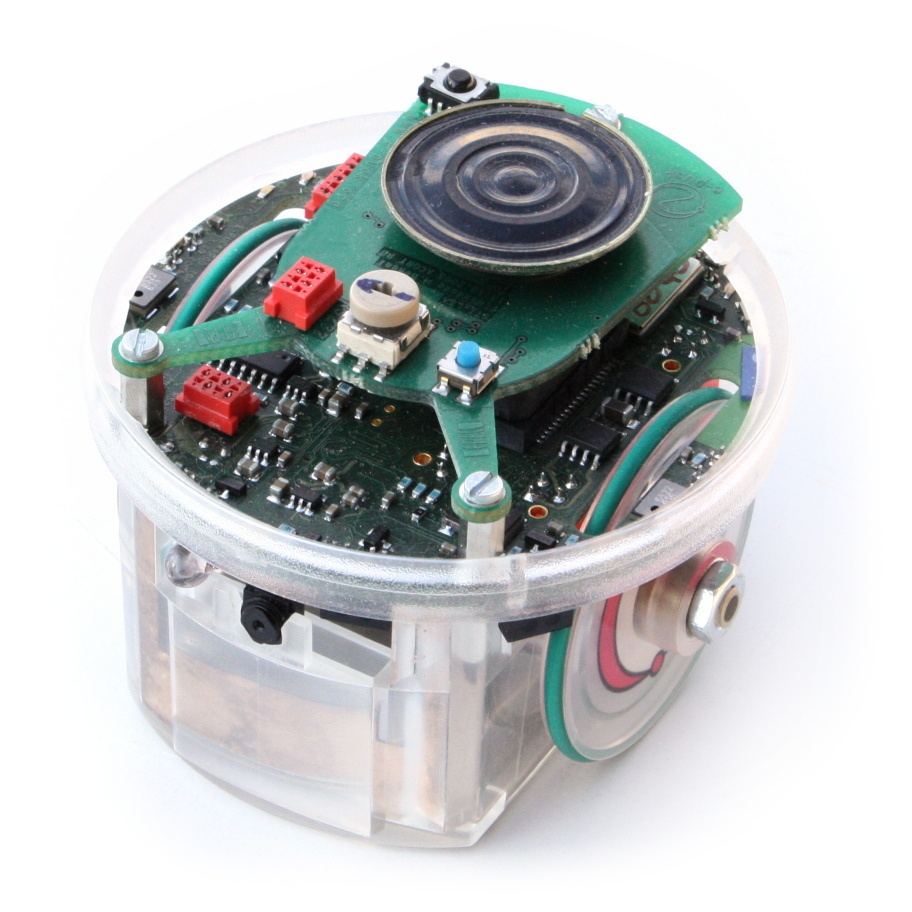
\includegraphics[width=0.7\textwidth]{./Figures/E-puck.jpg}
		\rule{35em}{0.5pt}
	\caption[swarm]{E-puck. Imagen extraida de Wikipedia}
	\label{fig:epuck}
\end{figure}

\textbf{Detalles técnicos}
\begin{itemize}
\item Diámetro: 70 mm
\item Alto: 50 mm
\item Peso: 200 g
\item Máxima velocidad: 13 cm/s
\item Autonomía: 2 horas moviéndose
\item dsPIC 30 CPU @ 30 MHz (15 MIPS)
\item 8 KB RAM
\item 144 KB Flash
\item 2 step motors
\item 8 sensores de proximidad y luz (TCRT1000)
\item color camera, 640x480
\item 8 LEDs en un aro +un LED en el cuerpo + un LED en frente
\item Acelerómetro 3D
\item 3 micrófono
\item 1 parlante
\end{itemize}

%-----------------------------------
%	SUBSECTION 4
%-----------------------------------

\subsection{3pi Robot}

Pololu, la misma marca que tiene desarrollo de varios tipos de motores para robótica y PCB para controlarlos, diseño el 3pi Robot. Es un robot bastante más económico que el e-puck, cuyo valor es 99.95USD ref. Sparkfun. También tiene dos ruedas para desplazarse de forma diferencial, 5 sensores de reflectancia, un LCD de 8x2 caracteres, un buzzer y tres botones para que el usuario pueda programarlos. Todos estos dispositivos están conectados a un microcontrolador ATmega328. Su velocidad es de 90 cm/s.

El 3pi fue diseñado especialmente como un robot seguidor de lineas y solucionador de laberintos. Existen varios videos que muestran la asombrosa velocidad de estos robots para solucionar un laberinto. Se programa en C, pero como posee un microcontrolador ATmega es posible hacer uso del bootloader Arduino y programarlo con ese IDE. Usa 4 baterias AAA y trae 4 LEDs.

Para el modelo que se planteó en este trabajo hace falta un módulo de comunicación inalámbrica, y el 3pi no tiene. Para usar esta alternativa es necesario sumarle a su precio 26USD, que es el precio del módulo XBee 1[w] serie 2 que se vende en Sparkfun.

\begin{figure}[htbp]
	\centering
		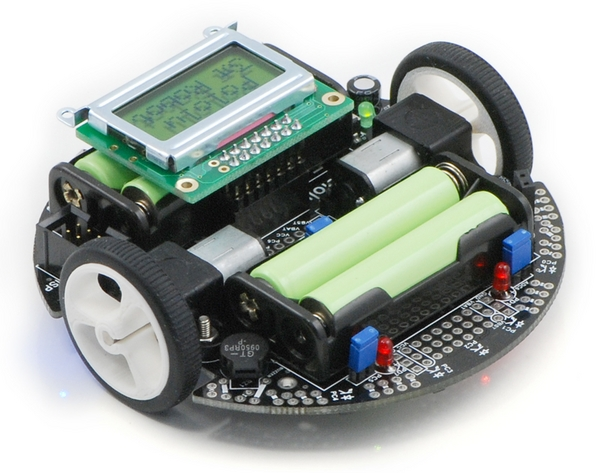
\includegraphics[width=0.7\textwidth]{./Figures/3pi.jpg}
		\rule{35em}{0.5pt} 
	\caption[swarm]{3pi Robot, simple y económico pero no tiene comunicación inalámbrica. Imagen extraida de http://www.skpang.co.uk}
	\label{fig:3pi}
\end{figure}

\textbf{Detalles técnicos}
\begin{itemize}
\item Procesador ATMega328
\item TB6612FNG Motor Driver
\item 2 canales de motores.
\item 3 - 7V voltaje de operación
\item 80kHz max PWM fequency
\end{itemize}

%-----------------------------------
%	SECTION 3
%-----------------------------------

\section{Necesidades de mercado}
\begin{figure}[htbp]
	\centering
		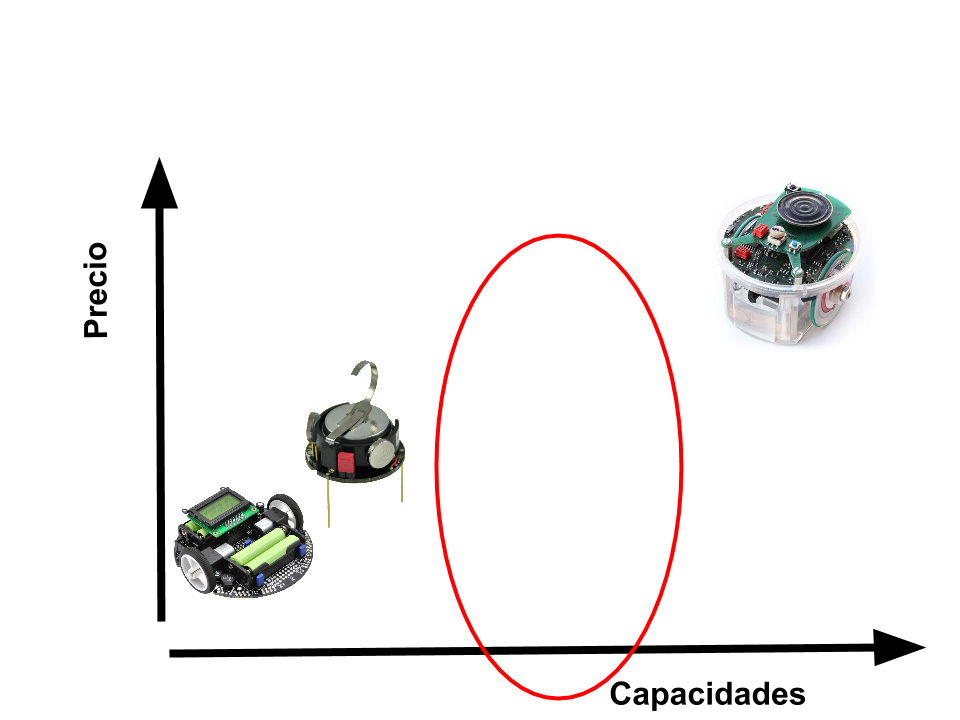
\includegraphics[width=0.8\textwidth]{./Figures/nicho.png}
		\rule{35em}{0.5pt}
	\caption[nicho]{Nicho de mercado}
	\label{fig:nicho}
\end{figure}

De los robots estudiados destaca en sus prestaciones el e-puck, pero este tiene dos grandes problemas para ser usado por gente que no es especialista en robots. Uno es que tiene demasiado hardware, lo que tiende a confundir y aumentar costos. Dos, que para su comunicación inalámbrica hace uso de Bluetooth, protocolo que no soporta las redes Mesh para hacer de manera simple el control de muchos dispositivos en una red. Hace falta un robot capaz de controlarse de forma inalámbrica, simple de construir y fácil de usar. Además debe ser económico para poder construir varios. Se pretende hacer uso de tecnologías como impresoras 3D y  de desarrollo como el Open Hardware.


%----------------------------------------------------------------------------------------
%	SUBSECTION 3
%----------------------------------------------------------------------------------------

\subsection{Usos Académico}

Un enjambre de robots puede presentar muchas ventajas dentro del aula. Si se tiene un sistema de fácil uso para los alumnos, el profesor puede asignar una tarea a un grupo de estudiantes donde cada uno tiene la responsabilidad de controlar o programar un robot para que el conjunto logre una meta determinada como ordenar unos bloques o hacerse cargo de regar un pequeño huerto. Abusando un poco del concepto de la colectividad, incluso pueden generarse tareas donde cada colegio se especializa en un tipo de tareas para luego juntar los distintos robots y probar cómo interactúan.

Tener un setup con robots que demuestren un comportamiento colectivo puede ser muy ventajoso para ayudar a niños con trastornos como el Asperger a practicar sus habilidades para reconocer estos mismo comportamientos.

\subsection{Usos Militar}

\subsection{Usos Doméstico}

